\documentclass[12pt, twoside]{article}
\usepackage[letterpaper, margin=1in, headsep=0.2in]{geometry}
\setlength{\headheight}{0.6in}
%\usepackage[english]{babel}
\usepackage[utf8]{inputenc}
\usepackage{microtype}
\usepackage{amsmath}
\usepackage{amssymb}
%\usepackage{amsfonts}
\usepackage{siunitx} %units in math. eg 20\milli\meter
\usepackage{yhmath} % for arcs, overparenth command
\usepackage{tikz} %graphics
\usetikzlibrary{quotes, angles}
\usepackage{graphicx} %consider setting \graphicspath{{images/}}
\usepackage{parskip} %no paragraph indent
\usepackage{enumitem}
\usepackage{multicol}
\usepackage{venndiagram}

\usepackage{fancyhdr}
\pagestyle{fancy}
\fancyhf{}
\renewcommand{\headrulewidth}{0pt} % disable the underline of the header
\raggedbottom
\hfuzz=2mm %suppresses overfull box warnings

\usepackage{hyperref}

\fancyhead[LE]{\thepage}
\fancyhead[RO]{\thepage \\ Name: \hspace{4cm} \,\\}
\fancyhead[LO]{BECA / Dr. Huson / Geometry\\*  Unit 5: Pythagorean theorem\\* 2 December 2022}

\begin{document}

\subsubsection*{5.5 Classwork: Pythagorean formula word problems}
\begin{enumerate}
\item Manuel takes a sheet of paper and cuts from one corner to the opposite corner, making two triangles. If the piece of paper is 12 centimeters long and 16 centimeters wide, how long is the diagonal cut that Manuel made?
\begin{flushright}
    \begin{tikzpicture}[scale=0.7]
    \node at (4,3)[above left]{$?$};
    \node at (8,3)[right]{12 cm};
    \node at (4,0)[below]{16 cm};
    \draw [thick] (0, 0)--(8, 0)--(8, 6)--(0,6)--cycle;
    \draw [dashed] (0, 0)--(8, 6);
    \draw [dashed] (8,0)++(-0.4,0)-- ++(0,0.4)-- +(0.4,0);
    \end{tikzpicture}
\end{flushright}

    
\item Three people are sitting on a bus. Lily is seated 12 feet directly behind Kelsey and 5 feet directly left of Alan. How far is Kelsey from Alan? \vspace{5cm}

\item A gopher has dug holes in opposite corners of a rectangular yard. One length of the yard is 9 meters and the distance between the gopher's holes is 15 meters. How wide is the yard?

\newpage
\item Three baseball players are playing catch. Brittany is directly south of Nancy and directly west of Gwen. Brittany and Gwen are 3 meters apart and Gwen and Nancy are 5 meters apart. How far apart are Brittany and Nancy? \vspace{4cm}
    
\item If the square of the hypotenuse of an isosceles right triangle is 128 $\text{cm}^2$, find the length of each side.
\begin{flushright}
  \begin{tikzpicture}[scale=1]
      \node at (3,3.2)[above left, rotate=45]{$c^2=128 \text{ cm}^2$};
      \node at (4,2)[right]{$x$};
      \node at (2,0)[below]{$x$};
      \draw [thick] (0, 0)--(4, 0)--(4, 4)--cycle;
      \draw [dashed] (4,0)++(-0.4,0)-- ++(0,0.4)-- +(0.4,0);
  \end{tikzpicture}
  \end{flushright} \vspace{2cm}

\item A ladder 13 meters long is placed on the ground in such a way that it touches the top of a vertical wall 12 m high. Find the distance of the foot of the ladder from the bottom of the wall.
\begin{flushright}
\begin{tikzpicture}[scale=1.2]
    \node at (0.8,2.3)[above left]{$13 \text{ m}$};
    \node at (2,2.5)[right]{$12 \text{ m}$};
    \node at (1,0)[below]{?};
    \draw [thick] (0, 0)--(2, 0)--(2, 5)--cycle;
    \draw [dashed] (2,0)++(-0.4,0)-- ++(0,0.4)-- +(0.4,0);
\end{tikzpicture}
\end{flushright}

\end{enumerate}
\end{document}